\documentclass[11pt]{article} 

../macros/macros.tex

\begin{document}

\newcommand{\LNabstract}{%
  These notes are for a typical undergraduate course on algorithms, covering the usual topics, but with more of an emphasis on learning to do proofs than is found in most courses.
  We take the perspective that being able to verify correctness (via detailed proofs)
  is an integral part of learning to design algorithms.}
\doTitle{1}{Preliminaries}{Preliminaries} 
\newpage

\section{External sources to complement these notes}\label{prelim: sec: textbooks}
\doHeader{Lecture notes and textbooks}

These lecture notes are meant as the primary reference material.
They are concise,
and they include the low-level details that lectures and textbooks often omit
in order to focus on developing intuition.

  \begin{figure}
    \begin{myframed}
\begin{description}\small

\item[(\hypertarget{source.DPV}{DPV})] \emph{Algorithms}, by Das Gupta, Papadimitriou, and Vazirani.  % \href
  % {https://www.amazon.com/Algorithms-Sanjoy-Dasgupta/dp/0073523402/ref=sr_1_fkmr0_1?keywords=Algorithms%2C+by+Das+Gupta%2C+Papadimitriou%2C+and+Vazirani&qid=1567179284&s=books&sr=1-1-fkmr0}
    % {(\$37)}

    pros: Concise, accessible, good for building intuition.  Drafts available online.
  \\ cons: So high level and informal that it hides many underlying details.
  

\item[(\href{https://jeffe.cs.illinois.edu/teaching/algorithms/}{JE})]
  \emph{Algorithms}, by Jeff Erickson.
  % \href
  % {https://www.amazon.com/dp/1792644833}
  % {(\$26)}
  % or
  {\small \url{https://jeffe.cs.illinois.edu/teaching/algorithms/}}

  pros: Individual chapters online. Articulates the thought processes behind the results.
  \\ cons: Relatively new.  Not yet widely used.  

\item[(\hypertarget{source.KT}{KT})] \emph{Algorithm Design}, by Kleinberg and Tardos.
  % \href
  % {https://www.amazon.com/Algorithm-Design-Jon-Kleinberg/dp/0321295358/ref=sr_1_1?keywords=Algorithm+Design%7D%2C+by+Kleinberg+and+Tardos&qid=1567179518&s=books&sr=1-1}
    % {(\$140)}
    
    pros: Provides motivation with modern examples.  Solutions to exercises can be found online.
    \\cons: Wordy and expensive. Solutions to all exercises can be found online.
    \\pro: lecture slides by K.~Wayne (KW):
  {\footnotesize \url{https://www.cs.princeton.edu/~wayne/kleinberg-tardos/}}
    
  \item[(\hypertarget{source.CLRS}{CLRS})] \emph{Introduction to Algorithms}, by Cormen et al.
    % \href
    % {https://www.amazon.com/Introduction-Algorithms-3rd-MIT-Press/dp/0262033844/ref=sr_1_fkmr0_1?keywords=Introduction+to+Algorithms%7D%2C+by+Cormen+et+al&qid=1567179625&s=books&sr=1-1-fkmr0}
      % {(\$82)}
    
      pros: Classic reference text.  Very thorough.  Widely used.  Soln's to some exercises are online.
      \\cons: A bit too thorough. Solutions to some exercises are online.
\end{description}

Those four are widely available.  We also refer to the following secondary sources:

\begin{description}\small


\item[(\href{https://courses.csail.mit.edu/6.042/spring18/mcs.pdf}{LLM})] \emph{Mathematics for Computer Science}, by Lehman, Leighton, and Meyer.
  Has a few good sections on proofs.
  \url{https://courses.csail.mit.edu/6.042/spring18/mcs.pdf}

\item[(\MF)] \emph{Building Blocks for Computer Science}, by Fleck.  Covers background material.
  \\
  \url{https://mfleck.cs.illinois.edu/building-blocks/}
  
\item[MIT lecture videos.] Available for some topics, mainly from these two courses:
  
  \parbox{0.8\textwidth}{
\url{https://ocw.mit.edu/courses/electrical-engineering-and-computer-science/6-006-introduction-to-algorithms-fall-2011/}
 \\[1ex] \url{https://ocw.mit.edu/courses/electrical-engineering-and-computer-science/6-046j-design-and-analysis-of-algorithms-spring-2015/}
}
\end{description}  
\vspace*{-10pt}
\end{myframed}
\caption{External sources to complement the lecture notes.  The four main sources are listed first.
  We recommend that you find one or two that suit you, and learn your way around them.}\label{prelim: fig: sources}
\end{figure}

% \paragraph{Online solutions.}
% For KT, a few exercises are solved in the text,
% and solutions to the rest (from the instructors manual) can be found online with some effort.
% For CLRS, solutions to some exercises from the \emph{second} edition (from the instructors manual)
% can be found online with some effort.

% \continued

On the other hand, the lecture notes are terse,
and provide neither motivation of the topic nor many examples.
These are important,
so we suggest that you complement your reading of the lecture notes
by using one or more sources in Figure~\ref{prelim: fig: sources}.
Please find copies online or at the library.
The various lecture notes will give more specific pointers into these resources.


\paragraph{Prerequisites.}
See Section~\ref{prelim: sec: background}
(and exercises in Section~\ref{prelim: sec: exercises})
for background topics you should know.

\newpage

\section{The 4-step recipe for presenting an algorithm}\doHeader{How to present an algorithm}
\doHeader{Presenting an algorithm}

Throughout these notes, we use the following 4-step recipe for presenting each algorithm:

\paragraph{1. Define the problem that the algorithm solves.}  Specify the possible inputs, and what the acceptable outputs are for each input.  Mathematically speaking, the problem definition defines a function mapping each input to a set of outputs.  For precision, the definition is typically given in terms of mathematically well-defined objects such as numbers, strings, trees, graphs, sequences, sets, etc.  The definition may introduce some problem-specific terminology for convenience.

\paragraph{2. Define the algorithm.}  Clearly specify the steps that the algorithm takes on any input.
 Describe the algorithm precisely in English, or pseudo-code if necessary for precision.
 Avoid giving code---algorithms are not programs.  They are read by people, not computers.
 A competent programmer should be able to easily translate your description into code.
 Learning to describe algorithms well is one of the main goals of these notes.
 Section~\ref{prelim: sec: algorithm} of this lecture note has more details.

\paragraph{3. Bound the worst-case run-time.}
  We model the worst-case run time as a function $T$ such that, for any positive integer $N$, $T(N)$ is the maximum, over all inputs of size $N$, of the number of steps the algorithm takes on that input.  Then we give big-O bounds on $T(N)$ in terms of $N$.
  
  The \emph{actual} number of steps in practice will depend on implementation details (for example: the programming language used, the compiler, and even the particular computer that the implementation runs on).  We want our analysis to be independent of these implementation details.  Generally speaking, these factors will affect the number of steps by at most some \emph{constant factor}.  Also, we are mainly concerned about the run-time for \emph{large} inputs.  For these reasons, we give big-O bounds---asymptotic bounds, neglecting constant factors and lower-order terms---on the run time.

\paragraph{4. Prove that the algorithm is correct.} (That is, for every input, it returns a correct output.)

In these notes, we model algorithms and the objects they work with mathematically.  That is, we define algorithms as well-defined processes that operate in a precise way on mathematical objects such as numbers, strings, trees, graphs, sequences, sets, and so on.  The advantage of this approach is \emph{precision}---when we think about or discuss an algorithm, we can understand, and agree on, precisely what we mean.  For example, we know precisely what we mean by an assertion such as ``Algorithm $A$ is correct'' (assuming Algorithm $A$ is itself well-defined).

A ``proof'' of such a statement is just a careful explanation of a precise line of reasoning by which it is clear that the statement is true (e.g., why, on \emph{every} possible input, the algorithm produces a correct output).  The guiding standard for written proofs is that, just by reading the proof, the intended reader should be able to \emph{easily} understand and verify that reasoning, step by step.  (As an aside: this means that the level of detail required in a proof depends on the intended reader.)

Learning to read and verify proofs about algorithms is another main goal.  As discussed later, learning to do this is similar to learning a new language and culture---proofs are expressed using various standard conventions, and to understand or present a proof you must know these conventions.  You'll need to immerse yourself in this language and culture.  At first, you may feel that you have been thrown into the deep end of the pool, but \emph{don't be intimidated}.  Many algorithms work in intuitively accessible ways, with intuitively accessible and familiar structures.  With exposure, as you learn the standard conventions and terminology, you will find algorithms, and reasoning about them, to be natural.

We'll do proofs in what we call \emph{long-form} format,
which is described in \LN{proofs}, on proofs.
Read that lecture note after this one.

% \newpage

\subsection{How to define an algorithm}\label{prelim: sec: algorithm}
\doHeader{How to define an algorithm}

% Recall the four steps for presenting an algorithm:

% \begin{mylist}
% \item[1.] Define the problem (input and output).
% \item[2.] Define the algorithm.
% \item[3.] Bound the worst-case asymptotic running time. 
% \item[4.] Prove correctness. 
% \end{mylist}

This section is about how to do the second step---defining the algorithm.
This step must present the algorithm in a precise and unambiguous way, so that from reading what is written the reader can know exactly what the algorithm does.  The definition should be (i) \emph{precise} and (ii) \emph{accessible} (easy to read).
For any competent programmer, translating the description into code in their favorite programming language should be a straightforward task.  Describing algorithms well takes a lot of practice.  Here is some guidance.

To achieve both precision and accessibility, you typically begin with an accessible, high-level description of the algorithm, to develop the reader's intuition for the main ideas.  This is written in English.  Depending on the algorithm, this could be a single sentence, a paragraph, or (for algorithms that are more complicated than those in these notes) a page or more.  This description should assume that the reader is a competent programmer (more on this below)
and is familiar with common algorithm-design techniques
(divide-and-conquer, dynamic programming, greedy algorithms, etc.).
Also, it should assume that the reader understands the problem definition.

But it is not always easy to give a description in English that specifies the details in a completely precise way.
If necessary, to make sure the details are clear, it often helps to follow the English description by \emph{pseudo-code}---for the algorithm or parts of it.  But what is pseudo-code?

\subsection{How to write pseudo-code}\label{prelim: sec: pseudo-code}\doHeader{Pseudo-code}

Think of pseudo-code as a high-level programming language, one designed to be read not by a computer, but by a \emph{competent programmer}.  Given the pseudo-code, the competent programmer should be able to ``compile'' the given algorithm into actual code in any programming language (an \emph{implementation} of the algorithm).   
But what knowledge can you assume that this programmer (the reader) has?
Don't assume that, a-priori, the reader knows anything about the algorithm you have in mind.
But you can assume the reader knows the following basics:
\begin{itemize}
\item The definition of the problem that the algorithm solves, including terminology defined there.
\item Programming constructs that are common to most programming languages:
\textsf{if-then-else} statements, \textsf{for} and \textsf{while} loops, function calls (including recursion), variables, assignment statements, and nested / indented code blocks.  Also, standard data types, including numbers, boolean values, strings, arrays, lists, dictionaries (e.g.~hash tables), and so on.
\item Standard mathematical objects (e.g., sets, sequences, trees, graphs)
  and standard mathematical notation (e.g.~logical and arithmetical operators, set notation, summations, quantifiers).
\item How to implement common programming sub-tasks, such as iterating over a collection of items, computing a sum,
  computing the maximum or minimum element in a collection, and so on.  Also, the worst-case asymptotic time that such a sub-task will take (e.g., $\Theta(n)$ time to iterate over a collection of $n$ items).
\end{itemize}

For the pseudo-code to be precise, it should have correct overall structure, and each line should have a clear and unambiguous meaning when read by any reader who knows the basics above.   To keep it accessible (easy to read and understand at a high level), it should judiciously \emph{omit low-level implementation details}.  But what details are okay to omit?  Any details that any reader (who knows the basics above) will be able to easily figure out.

\begin{figure}
  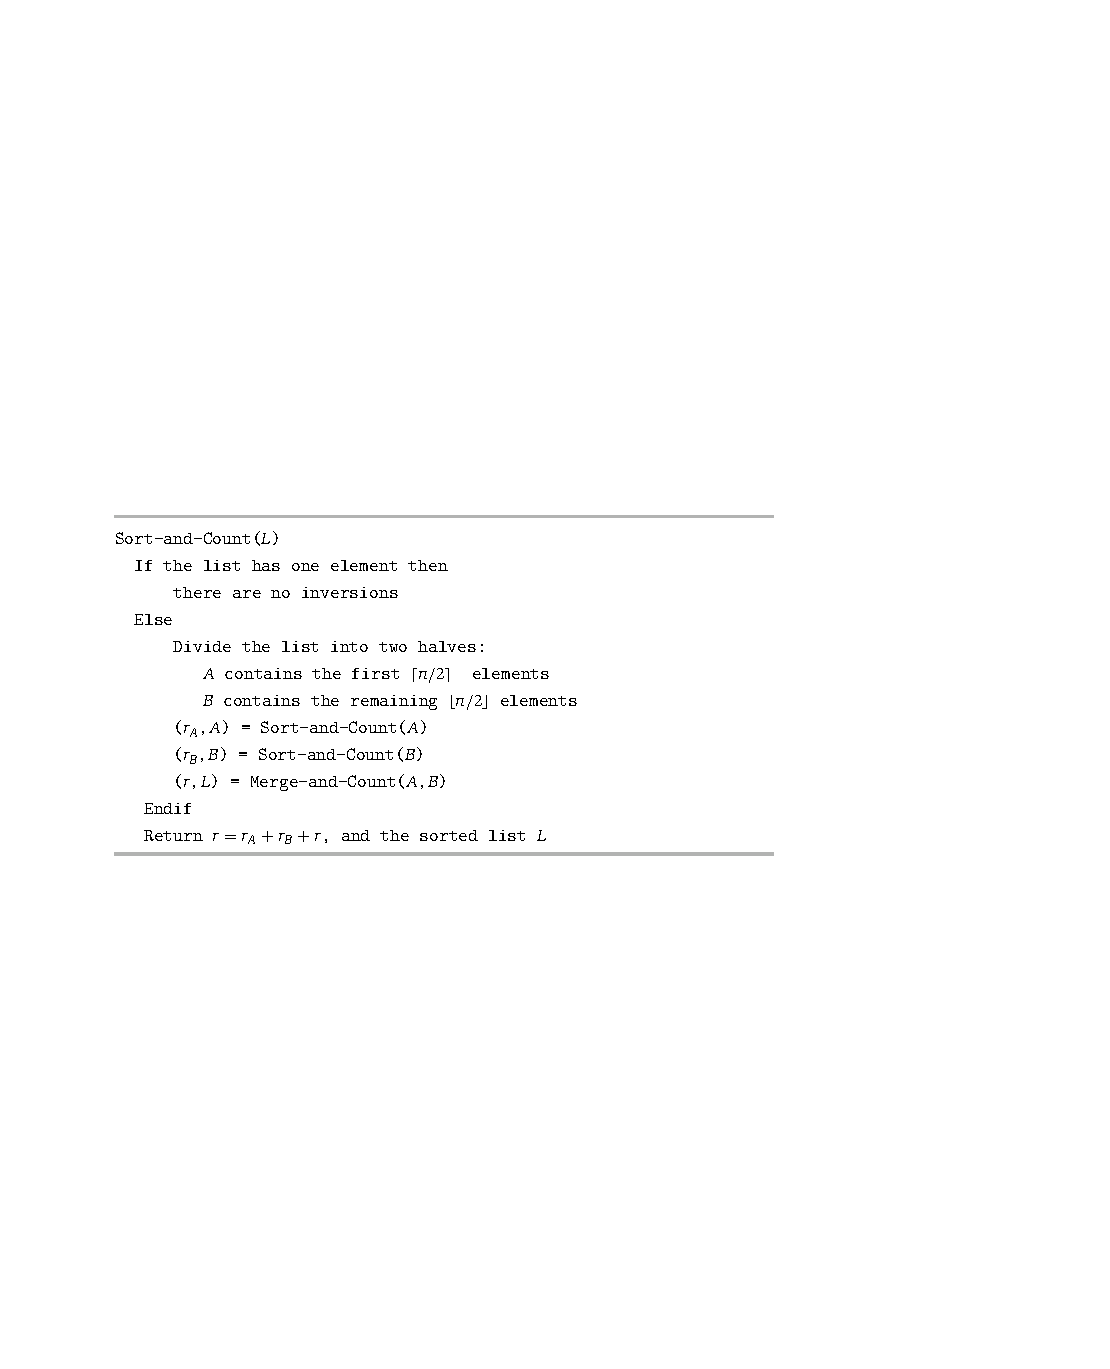
\includegraphics{KT-sort-and-count}\vspace*{-0.2in}
  \caption{Pseudo-code from \KT. (It also gives pseudo-code for \texttt{Merge-and-Count}, not shown.)
    This figure is \copyright\ the authors of \KT, reproduced here for commentary; it is not covered by these notes' license.}\label{prelim: fig: KT}
\end{figure}

 For example, see Figure~\ref{prelim: fig: KT}, which shows \KT's pseudo-code for an algorithm to count inversions.
 In that example, consider the statement starting with``\texttt{Divide the list into two halves:\ldots}''.  This description precisely defines the task to be solved. From reading just the description, any competent programmer should know how to write code that implements it.  So, it is okay that the low-level implementation details of this step are omitted.  Indeed, omitting them makes the description more accessible, because the low-level details would be distracting if present!  So, \emph{learn to use an appropriately high level of detail!}

\begin{figure}
  \begin{myframed}
    \begin{steps}\small
    \item[] \textsf{closest-pair}$(P=(p_1, p_2, \ldots, p_n))$
      \comment{($p_i=(x_i, y_i)\in \R^2$, with $x_1 < x_2 < \cdots < x_n$)}

      \step if $n \le 1$: return $\infty$
      \step if $n = 2$: return $d(p_1, p_2)$
      \step let $m = \lfloor n/2\rfloor$
      \step let $L = (p_1, p_2, \ldots, p_m)$;
      let $R = (p_{m+1}, \ldots, p_n)$
      \comment{(partition $P$ into left and right halves by x-coordinate)}
      \step let $\delta_L =  \textsf{closest-pair}(L)$; let $\delta_R =  \textsf{closest-pair}(R)$
      \step let $\delta = \min(\delta_L, \delta_R)$
      \step let $M = \{p_i : |x_i - x_m| \le \delta\}$
      \comment{(compute this in $O(n)$ time)}

      % [review 2026-09-27] fix: Step 8 set allowed i=j (so delta_M = 0) and had the typo y_j <= y_j + delta; added i != j and corrected to y_j <= y_i + delta
      \step let $\delta_M = \min\{ d(p_i, p_j) :\, p_i, p_j\in M, \, i \ne j, \, y_i \le y_j \le y_i + \delta\}$,  computed as described in the text

      \step return $\min(\delta, \delta_M)$
    \end{steps}
  \end{myframed}
\caption{Pseudo-code for finding the closest pair.
  \bookLink{latex.pseudocode}{Appendix B of the book} shows its LaTeX source.}\label{prelim: fig: closest pair}
\end{figure}

Mathematical language is, by design, very precise.
For this reason, mathematical language is very useful to precisely define relevant quantities.
Consider the example in Figure~\ref{prelim: fig: closest pair}.
In Step 7, mathematical notation is used to define $M$ as a set of points.
In Step 8, it is used to define $\delta_M$.\footnote
{However, in that step, because the actual method used to compute $\delta_M$ is complicated and requires further explanation, its implementation is described in the subsequent text, and Step 8 refers the reader to that description, which we don't repeat here.}
Assuming the reader is comfortable with mathematical notation, defining these quantities mathematically 
is much clearer than, say, giving a for loop that computes them.
So, \emph{learn to use mathematical notation and terminology correctly}!

We recommend that you use LaTeX to write up your solutions.
\bookLink{latex.homeworks}{Appendix B of the book} explains how to use LaTeX to prepare the homeworks,
including how to write pseudo-code with the macros that come with the homework templates.

\subsection{External sources on how to describe algorithms}
\begin{mylist}[-]
\item \JE Page 10,
  \href{https://jeffe.cs.illinois.edu/teaching/algorithms/book/!!-frontmatter.pdf}{Introduction} 0.5--0.7
\item \CLRS Page 16, Chapter 2.1 (but we prefer that you follow the style in the lecture notes here)
\end{mylist}

\vfill

% \continued 

% \section{Using Gradescope}

% \subsection{TODO}

% \continued 

\section{Meta-cognition to the rescue}
\doHeader{Meta-cognition to the rescue}

Some things to keep in mind, as we proceed, about learning algorithms

\subsection{Learning algorithms $\equiv$ learning a new language and culture}

When you are conversing or writing in a language that you are fluent in, you are generally able to focus on the high-level meaning that you want to convey, without being distracted by having to think about the lower-level mechanics such as grammar and vocabulary.  You internalized those lower-level mechanics through previous practice, and now they are automatic for you.

Learning to design and analyze algorithms is like learning a new language.  You start at the bottom of a learning curve, where even basic terms and concepts may be unfamiliar, and many aspects seem opaque.  You start by learning basic notation and terminology, and practice those until they become natural.  Then you learn the basic concepts, and work with them until they become natural.  As you practice, these building blocks become automatic for you.  You are no longer distracted by the lower-level details, and can focus on understanding algorithms at a higher level.  A similar process happens as you practice learning to communicate your ideas clearly.

You are also learning a new culture — the culture of a large ``algorithms'' community
with a rich history, a rich literature, and established (and useful) norms and language.

\paragraph{Immersion, feedback, and interaction.} 
The best way forward is to immerse yourself in it in some substantial way, to engage in regular, very focused practice, with lots of feedback and discussion as you go.
Your active engagement will come mostly from working on problems — spending hours thinking about them and struggling with them, and practicing communicating your ideas.

Make a special effort to get (and pay careful attention to) detailed feedback on your attempts.
Seek regular feedback from others: fellow students and, if you are taking a course, the course staff.
Feedback is crucial for discovering gaps in your understanding and in your explanations.
Feedback can also help you stay on track, and not waste as much time when you do have a gap or a roadblock.
Look particularly carefully at any feedback on work that you hand in. 

In this spirit, we encourage you to discuss the material, including your ideas for problems, with others who are learning it,
both to get help understanding the material, and to help others learn it.
Teaching others will increase your own understanding.
But if you are taking a course, follow its academic-integrity policy: typically you must write up your own solutions on your own, and you must not share your written solutions with other students!

\paragraph{But do your own pull-ups!}
Watching someone else do pull-ups won't make you stronger, and reading or hearing solutions won't make you good at solving problems.  The way to learn the material is to work through problems yourself, so engage fully with the exercises.

\paragraph{Meta-strategies for intuition in the face of abstraction.}
You will encounter many precise but abstract definitions of problems and algorithms.  Likewise, the proofs you'll see are given in full generality, and so are also abstract.  These definitions and proofs will condense a \emph{lot} of information and insight into a few terse lines, and their abstract nature may be a barrier to understanding.  Just reading them once is often not enough to develop a solid intuition for their meaning.

But maintaining an intuitive understanding is crucial!  To do that it helps to actively employ some meta-strategies:

\begin{enumerate}
\item Start by being mindful of when something (e.g., a definition) is not intuitive or is not clear for you.  When that happens, the first thing to do is slow down.  Review what you just read, or ask questions about what you just heard. Sit for a minute and consider it.   Consider a few specific examples.  Lectures and textbooks do this, and it's a good practice to do it on your own.  Often, drawing out an example, or a picture that represents the concept, helps.

\item
  A second meta-strategy:  Realize it takes your brain \emph{time to digest} new problems, algorithms, and lines of reasoning.  After you first read, say, a proof, or an algorithm, you may have a vague intuition for it, but you might not have digested it enough so that you understand all the pieces, or how they work together.  Put it aside for a while, think about something else, then come back to it. You may find that the material has become easier to work with.  It takes time for your brain to learn what's relevant.  Then opaque concepts can become clear.

\item
A third meta-strategy:  Talk it out with someone else.  Interacting (explaining and listening) engages your brain in ways that thinking on your own may not.  
\end{enumerate}

\paragraph{Start problems early.}
For the more challenging problems,
it may take a day or two just to digest the problem,
and then another day before you have some good ideas.
Your first tentative solutions are likely to have gaps or other errors that you can't see right away.
So, you may need to revisit your first drafts after a day or so to find and fix gaps or errors.
That is, there will be several phases: understanding the problem, coming up with ideas,
developing them, and checking and correcting them. Each phase will take time.
So, you should read the problems and start thinking about them early---if they are assigned in a course, at least a week before they are due for the harder problems---and then work on them again several times, a day or two apart.
If you can get help (for example, office hours or a discussion forum), consider using it in each phase---early on to get clarification on your understanding of the problem,
midway to get feedback on the direction you are pursuing,
and towards the end to get feedback on your full attempts.

\paragraph{Read lecture notes and do exercises before lecture.}
If you are attending lectures on this material, note that each lecture will cover lots of ground.  We will introduce a new problem, discuss one or more algorithms for it, then consider how to analyze those algorithms.  In short, we'll introduce several layers of concepts, each building on the previous.  This will be difficult to follow in real time if it is all new to you.  For this reason, we encourage you to read the lecture notes and do some of the easier exercises before the lecture, so you come to lecture already having some idea of the problem definitions and the algorithms we will do that day.  Then you will follow more easily when we get into the analysis.

\paragraph{Take-away: work hard to stay ahead of the curve!}
In short, it takes time to digest each new topic before it clicks.
As previous students have noted (see Section~\ref{prelim: sec: advice}), there is a risk of not having a topic click
until after the problems on it are due, or after an exam on it.
To avoid this, we strongly encourage you to stay ahead of the curve as much as possible.
Read lecture notes and do sample exercises at least a few days before the lecture on the topic.
Start each set of problems more than a week before it is due,
and continue to work on it in stages.
This way, by exam time, you will have had as much time as possible to digest the topics.
Also, when you have a time-consuming project in another course,
you will not be forced to do this work at the last minute.

\newpage

\subsection{Advice from previous students}\label{prelim: sec: advice}
% \doHeader{Advice from previous students}

At the end of a semester-long course based on these notes, students graciously left the following advice for future students:

\noindent \hrulefill 

1. Be honest with yourself and the professor when you don't understand something. At times I felt like because there were no questions from other people and I didn't understand a topic, that maybe everyone already understood it and I was simply behind. This might have been true sometimes, but the stress of snowballing into a topic that you don't understand is far greater than the stress of drawing a bit of attention for a reasonable question. In reference to the analogy of watching someone do pull-ups, just because a professor says something makes sense (especially with proofs), doesn't mean it actually makes sense to you. Proofs are complicated, so give yourself a break. Intuition takes time to build, not always just a lecture. The worst thing that can happen is that the professor will ask you to hold your question if there isn't enough time.

2. Procrastinating will not work for this class. I wish I didn't fight so hard against that fact, but it's simply impossible to determine how long an assignment will take you. There are too many variables that will affect your understanding of the homework for a course like this. It really just depends on what kinds of intuition you have coming into Algorithms. Sometimes it doesn't feel possible (as some people mentioned, we have various other difficult classes to deal with), but it does get easier with practice, and with support from your professors (most of them actually want you to succeed).

3. Review your data structures and practice with them. It didn't take me long to realize that just because I understand an algorithm, doesn't mean I can implement it efficiently. I do wish our semesters were long enough to cover implementations in more detail, but in the meantime, try to understand the things that make the algorithms click. Efficient programming will become important at one point if not now, so be sure that you're at least getting an idea of how things are implemented in actual code and why they work in practice vs theory. Again I'll refer to the pull-up analogy. This is something that I wish I had done more during the semester.

\noindent \hrulefill 

Form study group to revise by teaching each other, but complete the assignments independently. The former helped me to catch gaps in understanding and recall better in exams, the latter prepared me for exam condition. Go for office hour after coming up with a hand-written draft for the assignments, then format them in LaTeX afterward. Also, writing down a detailed cheat sheet helps.

\noindent \hrulefill 

1. Review the lecture notes for specific details on problems. More often than not, I would only get a high level understanding of the algorithms that were being discussed in class, and only understand them intuitively. The lecture notes have a lot of the specific details which actually put the higher level intuition of the algorithms into a concrete, logical, and provable concept.  
 
2. Get feedback on the homeworks after they are graded. Sometimes when I got homework back, I sort of realized what I did wrong but didn't take the time to fully understand why I got points taken off. Usually it was for small details that were crucial to the proofs or correctness of an algorithm, which can make or break a problem. This also helped when preparing for the midterms or the final exam.


\newpage % \continued

\section{Background topics to review}\doHeader{Background}\label{prelim: sec: background}

We assume that from the prerequisite courses you already know various background topics such as
how to program, recursion, sorting algorithms (e.g.~mergesort), basic data structures
(e.g.~hash tables, heaps, binary search trees, graphs),
and basic discrete math: proof, induction, asymptotic (big-O) notation, 
set notation, summation notation, quantifiers,
basic properties of logarithms, polynomials, and exponential functions,
doing algebra with inequalities, and so on.

% \subsection{Basic math reference}\label{prelim: sec: math ref}%\doHeader{Math reference}
Below, for reference, are definitions and properties of the big-O notations,
and some properties of logarithms that you may want to know.
Sources for reviewing other background material are listed at the end of this section. 

\subsection{Big-O notation definitions and useful rules of thumb}\label{prelim: sec: big-O}

Here are formal definitions of the big-O, big-$\Omega$, and big-$\Theta$ notations.
You'll need them for the exercises.

\begin{definition} Fix any two functions $f, g:\R\rightarrow \R$. 
  \begin{mylist}[$\bullet$]
  \item $f(n) = O(g(n))$ if there are positive constants $c, n_0 > 0$ such that,
  for all $n \ge n_0$,
  \[ 0 \le f(n) \le c\, g(n). \]

\item  $f(n) = \Omega(g(n))$ if $g(n)$ is $O(f(n))$.  Equivalently,
  there are $c, n_0>0$ such that, for all $n \ge n_0$,
  \[ f(n) \ge c\, g(n) \ge 0. \]

\item  $f(n) = \Theta(g(n))$ if $f(n)$ is $O(g(n))$ and $f(n)$ is $\Omega(g(n))$.
  Equivalently, there are $c_1, c_2, n_0>0$ such that, for all $n \ge n_0$,
  \[ 0 \le c_1\, g(n) \le f(n) \le c_2\, g(n). \]
\end{mylist}
\end{definition}

\paragraph{Two rules of thumb for easy cases:}~

You can use the limit of the ratio $f/g$ to determine the big-O relationship, when the limit exists:

\begin{lemma}\label{prelim: lemma: ratio}
  Suppose $f(n)$ and $g(n)$ are non-negative for all sufficiently large $n$,
  and the limit $\ell = \lim_{n\rightarrow\infty} f(n)/g(n)$ exists.
  Then
  \begin{mylist}[$\bullet$]
  \item $f(n) = O(g(n))$ if and only if $\ell < \infty$
  \item $f(n) = \Omega(g(n))$ if and only if $\ell > 0$
  \item $f(n) = \Theta(g(n))$ if and only if $0 < \ell < \infty$
  \end{mylist}
\end{lemma}

\continued

Most functions we deal with will have just just logarithmic, polynomial, and exponential terms.
The next rule of thumb makes it easy to determine the big-O relationships between such functions.

\begin{lemma}\label{prelim: lemma: general}
Suppose, for some constants $a, b, c, a', b', c' \in\R$ (with $a,a'>0$), that
\begin{align*}
  f(n) &{} = a^n \times n^b \times \log^c n \text{~~and~} \\
  g(n)&{} =  (a')^n \times n^{b'} \times \log^{c'} n.
\end{align*}
Then $f(n) = O(g(n))$ if and only if $(a, b, c)$ is lexicographically at most $(a', b', c')$.  That is, iff
\begin{mylist}[$\bullet$]
\item $a < a'$, or
\item $a = a'$ and $b < b'$, or
\item $a = a'$, $b = b'$, and $c \le c'$.
\end{mylist}
\end{lemma}

For example, $n^3\log^2 n = O(n^{3.1})$, but $n^3\log^2 n \ne O(n^{3})$.

And $2^n = O(3^n/n^3)$, but $2^n \ne O(2^n / n^3)$.

We omit the proofs of these lemmas, but here is the idea for Lemma~\ref{prelim: lemma: general}.
Following Lemma~\ref{prelim: lemma: ratio} consider the limit of the ratio:
\[
  \lim_{n\rightarrow\infty} \frac{f(n)}{g(n)}
  =
  \lim_{n\rightarrow\infty} \log^{c-c'}_2(n)\, n^{b-b'}\, \Big(\frac{a}{a'}\Big)^n.
\]
This limit exists and (by calculation) is finite if and only if the given condition holds.

\subsection{Properties of logarithms that are good to know}\label{prelim: sec: logarithms}

% [review 2026-09-27] fix: the logarithm identities need the bases to be != 1; added the side condition b, c != 1 where they appear as bases
For all $a, b, c > 0$ (with $b, c \ne 1$ wherever they appear as bases):

\begin{enumerate}
\item \(\log_b (ac) = \log_b a~+~\log_b c\)

\item \(\log_b (a^c) = c\,\log_b a\)

\item \(\log_b a = \log_c a / \log_c b\)  \comment{\ldots change of base}

\item $b^{\log_c a} = a^{\log_c b}$\comment{\ldots often useful for recurrence relations}

% [review 2026-09-27] fix: a! requires a to be a positive integer; added that side condition
\item $\log (a!) = \Theta(a\log a)$ for positive integers $a$  \comment{\ldots because $(a/2)^{a/2} \le a! \le a^a$}
  
\end{enumerate}

\subsection{External sources on background material}
\begin{mylist}[-]

\item \DPV Chapter 0 (algorithms, big-O notation)

\item JE
  \href{https://jeffe.cs.illinois.edu/teaching/algorithms/book/!!-frontmatter.pdf}{Preface}
  (has a detailed list of background topics and further reading), and
  \href{https://jeffe.cs.illinois.edu/teaching/algorithms/book/00-intro.pdf}{Introduction}

\item \KT Chapters 1 (algorithms) and 2 (big-O notation).
  (See also the \KWSlides for those chapters.)

\item \CLRS Chapters 1 \& 2 (algorithms), 3 (big-O notation), Appendices A and B (basic math)

\item \MF, especially
  \begin{mylist}
  \item
    \href{https://mfleck.cs.illinois.edu/building-blocks/version-1.3/math-review.pdf}{Chapter 1: Math Review}
  \item
    \href{https://mfleck.cs.illinois.edu/building-blocks/version-1.3/proofs.pdf}{Chapter 3: Proofs}
  \item
    \href{https://mfleck.cs.illinois.edu/building-blocks/version-1.3/induction.pdf}{Chapter 11: Induction}
  \item
    \href{https://mfleck.cs.illinois.edu/building-blocks/version-1.3/big-o.pdf}{Chapter 14: Big-O}
  \item
    \href{https://mfleck.cs.illinois.edu/building-blocks/version-1.3/algorithms.pdf}{Chapter 15: Algorithms}
  \end{mylist}
  
\end{mylist}

% \continued

\section{Exercises on background topics}\label{prelim: sec: exercises}\doHeader{Exercises}

\subsection{Exercises with solutions}

\paragraph{External problems with solutions}
\begin{mylist}[-]
\item \KT Page 65, Solved Exercises 1 and 2 (big-O notation)
% \item \MF
\end{mylist}

%%%%%%%%%%%%%%%% PROBLEM %%%%%%%%%%%%%%%%%

\exercise \emph{(Big-O notation, proof)}
Suppose $f(n)$, $g(n)$, and $h(n)$ are non-negative functions with $f(n) = O(h(n))$ and $g(n) = O(h(n))$.
Use the definition of big-O in \LN{prelim} to prove that $f(n)+g(n) = O(h(n))$.
Give this proof in long form (as described in \LN{proofs} on proofs).
Be careful to get your reasoning about the quantifiers (in the definitions of big-O) right.

\solution

\begin{longFormProof}

  \step Consider any functions $f$, $g$, and $h$ as described in the theorem.

  \step Let constants $c_1, n_1>0$ be such that
  $(\forall n \ge n_1)~ f(n) \le c_1\, h(n)$.  (These exist by def'n of big-O.)
  
  \step Likewise, let constants $c_2, n_2>0$ be such that
  $(\forall n \ge n_2)~ g(n) \le c_2\, h(n)$.

  \step Fix $n_3 = \max\{n_1, n_2\}$ and $c_3 = c_1 + c_2$.

  \step By algebra and the previous steps, then, $(\forall n \ge n_3)~ f(n) + g(n) \le c_3 \,h(n)$.

  \step Therefore, by the definition of big-O, $f(n) + g(n) = O(h(n))$. 
  
\end{longFormProof}

Alternative proof with explicit ``for all'' block (a little more detail than necessary):

\begin{longFormProof}

  \step Consider any functions $f$, $g$, and $h$ as described in the theorem.

  \step Let constants $c_1, n_1>0$ be such that
  $(\forall n \ge n_1)~ f(n) \le c_1\, h(n)$.  (These exist by def'n of big-O.)
  
  \step Likewise, let constants $c_2, n_2>0$ be such that
  $(\forall n \ge n_2)~ g(n) \le c_2\, h(n)$.

  \step Fix $n_3 = \max\{n_1, n_2\}$ and $c_3 = c_1 + c_2$.

  \begin{block}\label{prelim: block: O forall}
    \step Consider any $n\ge n_3$.

    \step Since $n_3 \ge n_1$,  $f(n) \le c_1 h(n)$. 

    \step Since $n_3 \ge n_2$,  $g(n) \le c_2 h(n)$.

    \step By algebra, $f(n) + g(n) \le (c_1 + c_2) h(n) = c_3 h(n)$.
  \end{block}    

  \step By Block~\ref{prelim: block: O forall}, for all $n \ge n_3$, we have $f(n) + g(n) \le c_3 \,h(n)$.

  \step Therefore, by the definition of big-O, $f(n) + g(n) = O(h(n))$. 
  
\end{longFormProof}

\subsection{Exercises without solutions}
%%%%%%%%%%%%%%%% PROBLEM %%%%%%%%%%%%%%%%%

\exercise \emph{(Big-O notation)}
Give the asymptotic values of the following functions, using the $\Theta$-notation.
Give the simplest possible answer.
%
%
\begin{enumerate}[label=(\alph*)]
\item $\frac{1}{2} n^5 + 7 n^4 - n^3 + 13n$
\item $3 + 2n^{-2} + 1/(\log^2 n)$
\item $n ( 7n^3\log n + 9 n\log^5n) + 15n^3$
\item $n^2 2^n + 13n^4 + n^3\log n$
\item $n^5 3^n + n 4^n$
\end{enumerate}
% 

%%%%%%%%%%%%%%%% PROBLEM %%%%%%%%%%%%%%%%%

\exercise \emph{(Big-O notation. Similar to Solved Exercise 1, \KT Page 65.)}
Rank the following functions in increasing order of asymptotic growth rate.
That is, reorder the functions so that each function is big-O of the following function.
No justification is required.

\newcommand{\sep}{~~~~}

\[
  n^3
  \sep
  7^{\log_2 n}
  \sep 
  n!
  \sep 
  12^n
  \sep 
  \log_2 (n!)  
  \sep 
  2^{4n}
  \sep 
  100 n^{3/2}
  \sep 
  10n
  \sep 
  2^{\log_3 n}
  \sep 
  \log_2^3 n
\]

%%%%%%%%%%%%%%%% PROBLEM (INDUCTION) %%%%%%%%%%%%%%%%%

\exercise \emph{(Induction and recursion)}
You encounter the following mysterious piece of code.

\begin{myframed}
  \begin{steps}
  \item[] def $C(a,n)$:
    \step if  $n=0$: return $(1,a)$
    \step let $(u,w) = C(a, \lfloor n/2 \rfloor)$
    \step if $n$ is even:  return $(u \cdot u, u \cdot w)$
    \step if $n$ is odd: return $(u \cdot w, w \cdot w)$
  \end{steps}
\end{myframed}

\begin{enumerate}[label=(\alph*)]
\item What are the outputs of $C(a, 1)$, $C(a,2)$, $C(a,3)$, and $C(a,4)$ (in terms of $a$)?  You do not need to justify your answers.

\item Give a closed-form expression (in terms of $a$ and $n$) for the value output by $C(a,n)$,
  assuming $n$ and $a$ are non-negative integers.

\item 
  Prove by induction on $n \ge 0$ that $C(a,n)$ indeed outputs the value you gave.

\item Prove that for each positive integer $n$, during the execution of $C(a,n)$,
  it does at most $2 + 2 \cdot \log_2 n$ multiplications.
\end{enumerate}

\paragraph{External exercises without solutions}\!\!\!\!\!\footnote
{As mentioned in Section~\ref{prelim: sec: textbooks},
  solutions for exercises in \KT, and some exercises in \CLRS, can be found online.}
\begin{mylist}[-]
\item \KT Page 67, Exercises 1 through 8
\item \CLRS Page 52, Exercises  3.1--1 through 3.1--8
\item \DPV Page 18, Exercises 0.1 through 0.3
\end{mylist}

\end{document}

%%% Local Variables:
%%% mode: latex
%%% TeX-master: t
%%% End:
